\documentclass{article}
\usepackage{graphicx} % Required for inserting images
\title{synchronous counter}
\begin{document}
\maketitle
 \begin{enumerate}     
  \item A 2-bit synchronous counter using two J-K flip flops is shown. The expressions for the inputs to the J-K flip flops are also shown in the figure. The output sequence of the counter starting from $Q_1Q_2 = 00$ is 
    \begin{figure}[!ht]
        \centering
        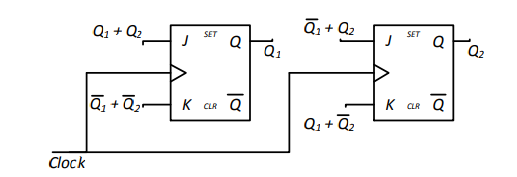
\includegraphics[width=\columnwidth]{/sdcard/internship/latex/figs/question44.png}
        \caption{$2$-bit synchronous counter}
        \label{fig:enter-label}
    \end{figure}
    \begin{enumerate}
        \item $00\rightarrow11\rightarrow10\rightarrow01\rightarrow00...$ 
        \item $00\rightarrow01\rightarrow10\rightarrow11\rightarrow00...$
        \item $00\rightarrow01\rightarrow11\rightarrow10\rightarrow00...$
        \item $00\rightarrow10\rightarrow11\rightarrow01\rightarrow00...$
    \end{enumerate}
    \end{enumerate }
\end{document}
